\documentclass{standalone}

%----------------------------------------------------------------------------------------------%
%                                 Packages and basic declarations
%----------------------------------------------------------------------------------------------%

\usepackage[utf8]{inputenc}
\usepackage{pgfplots}
\usepackage{tikz}


%----------------------------------------------------------------------------------------------%
%----------------------------------------------------------------------------------------------%
%                                            DOCUMENT STARTS
%----------------------------------------------------------------------------------------------%
%----------------------------------------------------------------------------------------------%

\begin{document}


%Tikz picture starts%

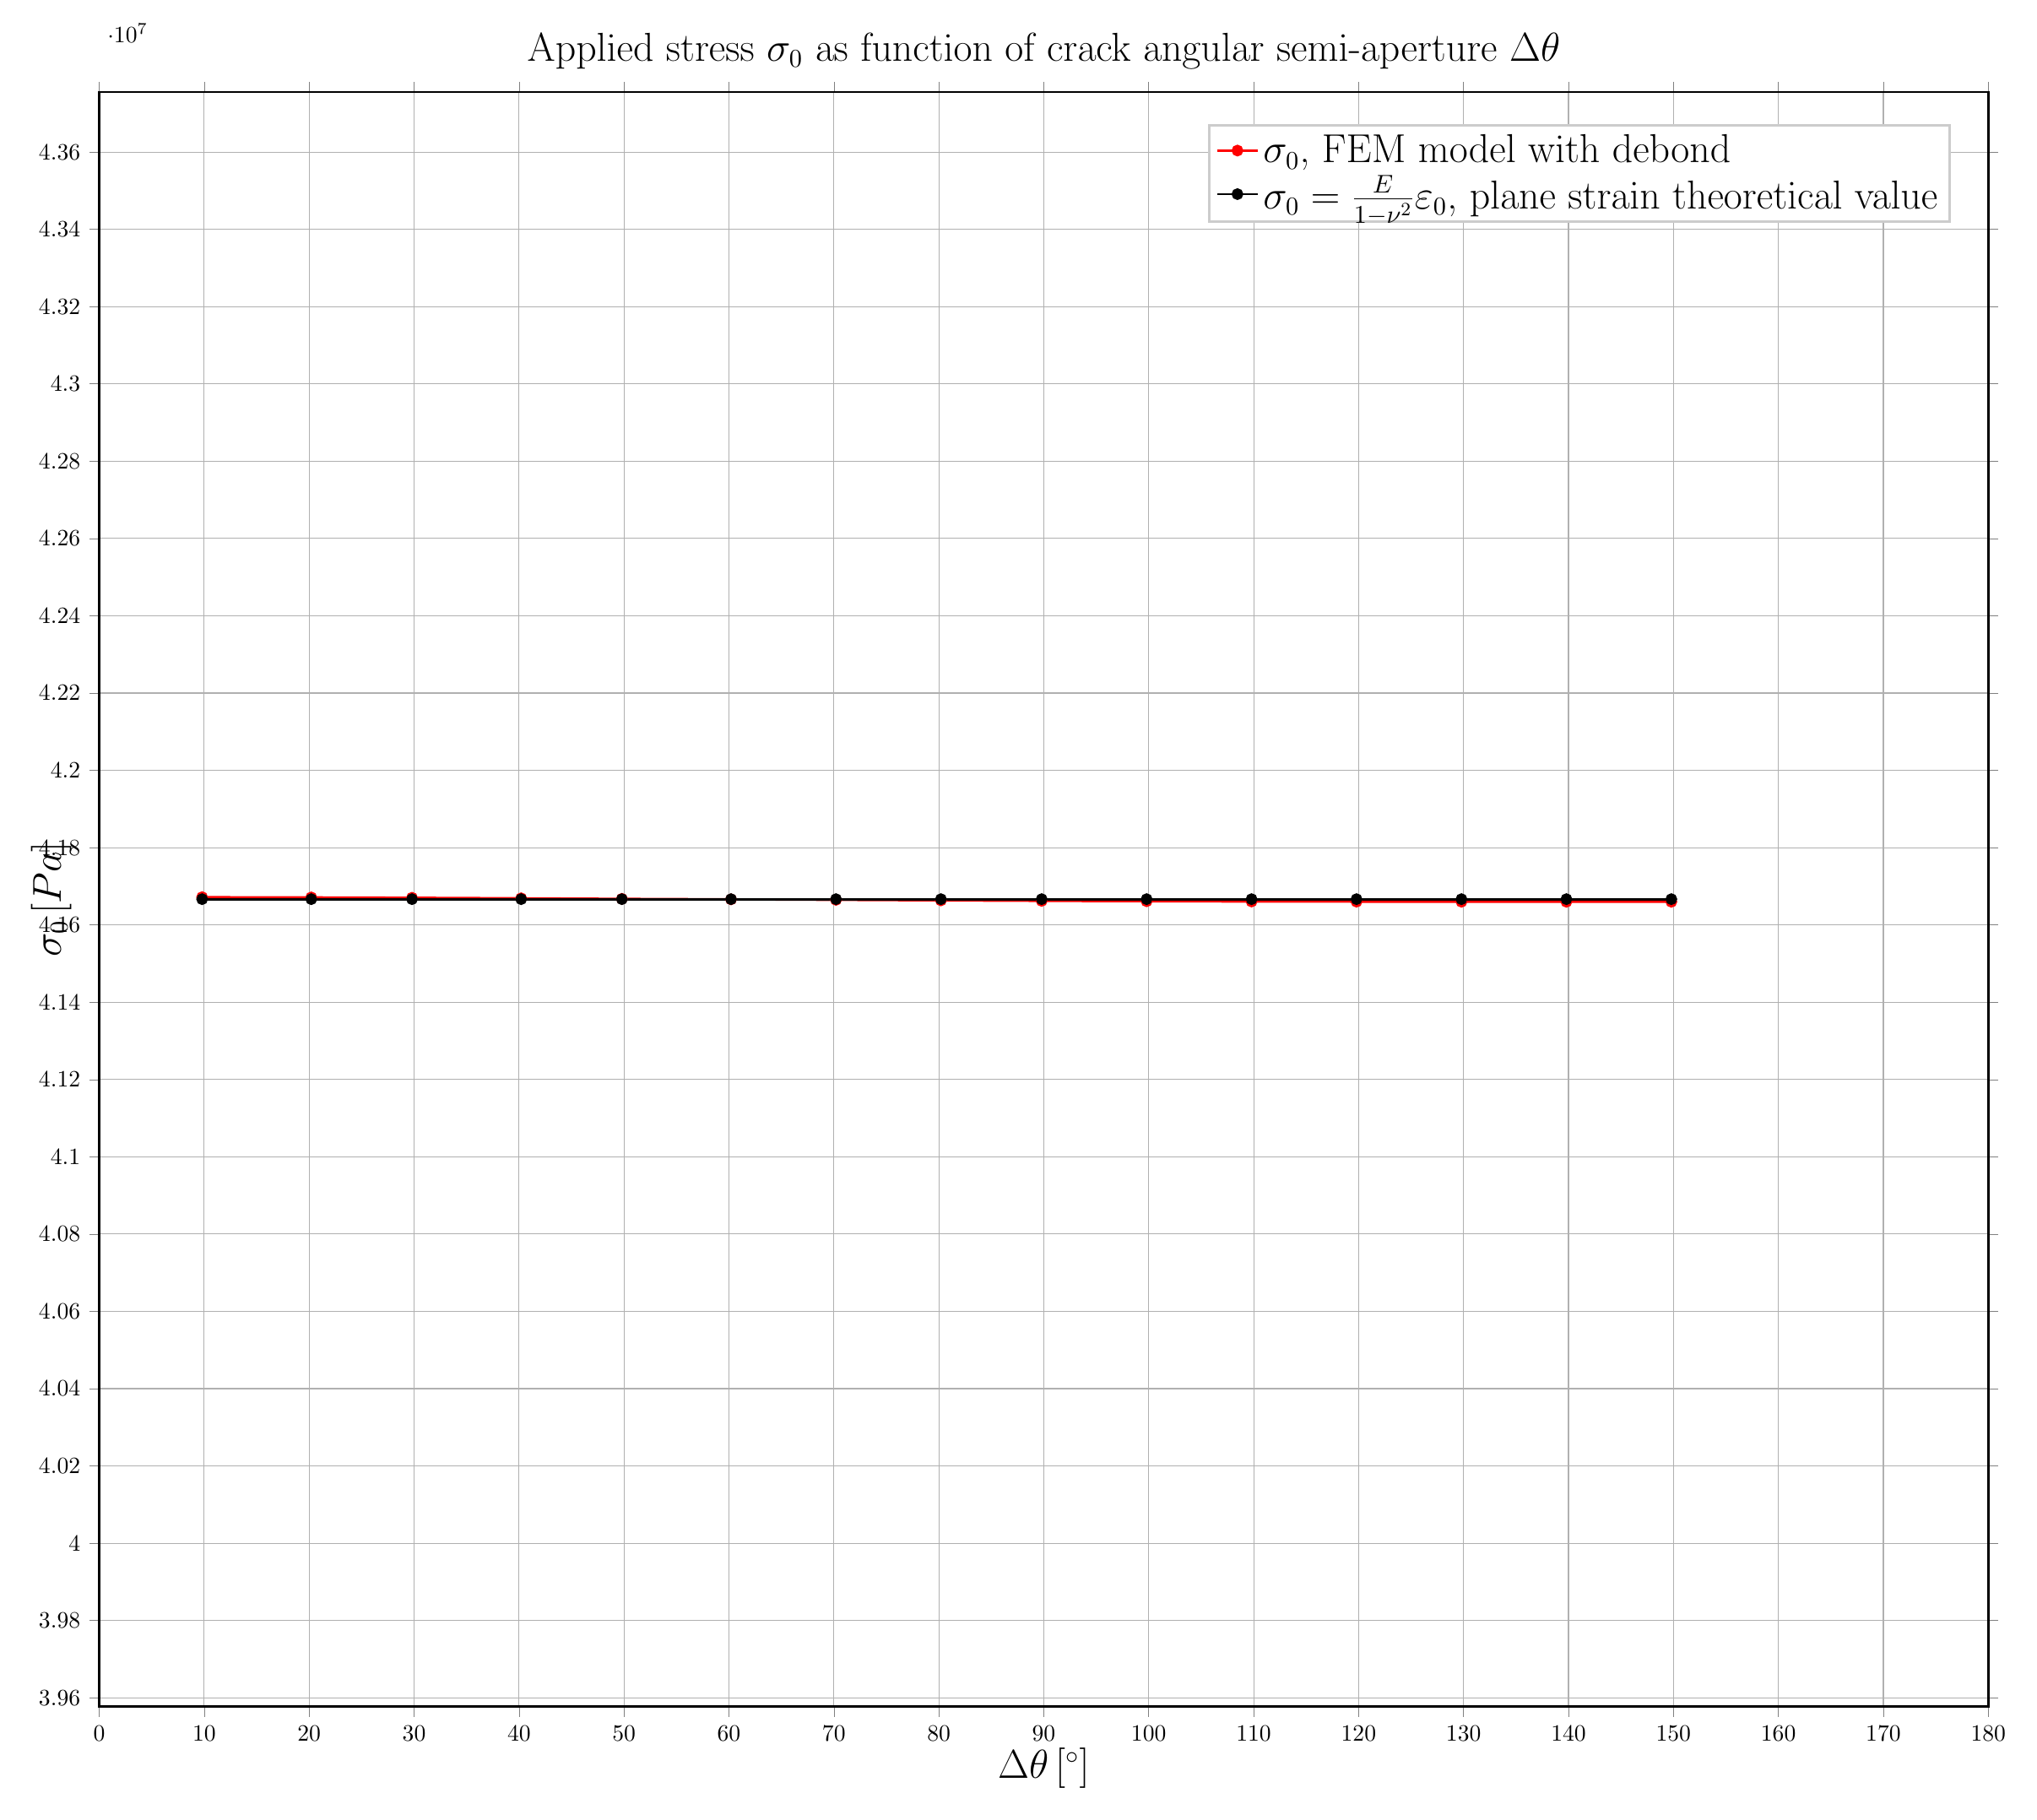
\begin{tikzpicture}

%Tikz axis starts%

\begin{axis}[width=30cm,
title={Applied stress $\sigma_{0}$ as function of crack angular semi-aperture  $\Delta\theta$},
title style={font=\fontsize{16}{8}\selectfont},
xlabel style={at={(axis description cs:0.5,-0.02)},anchor=north,font=\fontsize{16}{8}\selectfont},
ylabel style={at={(axis description cs:-0.01,.5)},anchor=south,font=\fontsize{16}{8}\selectfont},
xlabel={$\Delta\theta\left[^{\circ}\right]$},ylabel={$\sigma_{0}\left[Pa\right]$},
xmin=0.0,
xmax=180.0,
ymin=39576909.1197,
ymax=43755364.2011,
tick align=outside,
tick label style={font=\normalsize},
xtick={0.0,10.0,20.0,30.0,40.0,50.0,60.0,70.0,80.0,90.0,100.0,110.0,120.0,130.0,140.0,150.0,160.0,170.0,180.0},
xmajorgrids,
x grid style={lightgray!92.026143790849673!black},
ymajorgrids,
y grid style={lightgray!92.026143790849673!black},
line width=0.35mm,
legend style={draw=white!80.0!black,font=\fontsize{16}{12}\selectfont},
legend entries={{$\sigma_{0}$, FEM model with debond},{$\sigma_{0}=\frac{E}{1-\nu^{2}}\varepsilon_{0}$, plane strain theoretical value}},
legend cell align={left}
]

\addplot[red,smooth,mark=*]
table{
9.8000083551 41671775.4296
20.2001564043 41671173.6021
29.7996713865 41670270.0758
40.1999526243 41668915.0144
49.8000464651 41667494.1915
60.2003242878 41666213.4913
70.1998714969 41664831.8029
80.1999924418 41663442.1475
89.799994075 41662219.7016
99.8000057369 41661242.8733
109.800126682 41660554.9281
119.799673891 41660162.2421
129.800136345 41659984.6393
139.800052385 41659923.4269
149.799859141 41659920.971
};

\addplot[black,smooth,mark=*]
table{
9.8000083551 41666666.6667
20.2001564043 41666666.6667
29.7996713865 41666666.6667
40.1999526243 41666666.6667
49.8000464651 41666666.6667
60.2003242878 41666666.6667
70.1998714969 41666666.6667
80.1999924418 41666666.6667
89.799994075 41666666.6667
99.8000057369 41666666.6667
109.800126682 41666666.6667
119.799673891 41666666.6667
129.800136345 41666666.6667
139.800052385 41666666.6667
149.799859141 41666666.6667
};

\end{axis}
%Tikz axis ends%


\end{tikzpicture}
%Tikz picture ends%


\end{document}

%----------------------------------------------------------------------------------------------%
%----------------------------------------------------------------------------------------------%
%                                            DOCUMENT ENDS
%----------------------------------------------------------------------------------------------%
%----------------------------------------------------------------------------------------------%

